%%%%%%%%%%%%%%%%%%%%%%%%%%%%%%%%%%%%%%%%%%%%%%%%%%%%%%%%%%%%%%%%%%%%%%%%%%%%%%%%%%%%%%%%
\chapter[Correlations in Kitaev Spin Liquids]{Correlations in\linebreak Kitaev Spin Liquids}
\label{chapter:SpinCorrelationsOfKSL}
%%%%%%%%%%%%%%%%%%%%%%%%%%%%%%%%%%%%%%%%%%%%%%%%%%%%%%%%%%%%%%%%%%%%%%%%%%%%%%%%%%%%%%%%
%
%
The last two chapters demonstrated that Kitaev's honeycomb model hosts a broad diversity of gapless quantum spin liquid states when extended to various two- and three-dimensional tricoordinated lattices.
This chapter will explore the consequences which the corresponding gapless modes have on certain equal-time correlation functions of spins.
The focus will be on the spin-spin correlation functions briefly mentioned in Chapter~\ref{chapter:KitaevHoneycombModel} as well as a certain four-spin correlation function, referred to here as the bond-bond correlation function.

While the spin-spin correlations vanish beyond nearest-neighbors, at finite temperature the buildup of these correlations signals a thermodynamic crossover associated to the itinerant Majorana fermions.
The bond-bond correlations, however, intimately reflect the gapless nature of the spin liquids.
Whereas bond-bond correlations are short-ranged in the gapped spin liquid phases, in the \textit{gapless} spin liquid phases the correlation function decays algebraically in a way that depends both on the dimension of the lattice \textit{and} on the character of the gapless modes.
Recently, these bond-bond correlations between pairs of bonds in distinct bipartitions of a honeycomb lattice have been shown to be related to the entanglement entropy~\cite{YangARXIV2019}.
In particular, the quantity obtained by integrating the bond-bond correlation function $\avg{Q_A Q_B} - \avg{Q_A} \avg{Q_B}$ over all bonds $Q$ in the respective bipartitions $A$ and $B$ exhibits the same scaling law as the fermionic contribution to the entanglement entropy for the same bipartition.

It has long been known that the Kitaev honeycomb model defined for \textit{classical} Heisenberg spins hosts a classical spin liquid ground state which can be mapped to a hardcore dimer model.
The classical Kitaev spin liquid also boasts extremely short-ranged spin-spin correlations as well as algebraically decaying bond-bond correlations.
The origin of these algebraic correlations, however, is very different as classical Kitaev spin liquids obviously do not host gapless fermions.
Instead, these correlations are seen to decay in a manner which depends only on the dimension of the underlying lattice.
In Section~\ref{section:chapter07_ClassicalCorrelations}, a very brief introduction to the classical Kitaev model is given along with a discussion of the origins of short-ranged spin-spin correlations and algebraic bond-bond correlations in order to contrast the results of the quantum model.

The rest of this chapter reports on an ongoing study of correlation functions of spins in the \textit{quantum} Kitaev spin liquids.
Section~\ref{section:chapter07_SpinSpinCorrelations} explores the short-ranged spin-spin correlations at both zero temperature and finite temperature, comparing both analytic and numeric results.
Section~\ref{section:chapter07_BondBondCorrelationsZeroTemperature} gives a rather lengthy analysis of the bond-bond correlation functions at zero temperature.
Numerical calculations of bond-bond correlations are presented for a number of two- and three-dimensional lattices for spin liquids hosting Dirac nodes, Fermi lines in two- and three-dimensions, fully two-dimensional Fermi surfaces and Weyl nodes.
A long wavelength analysis is carried out in detail for the two-dimensional lattices to extract the algebraic decay and accompanying Friedel oscillations of the bond-bond correlation function, providing quantitative agreement with the numerics.
Some general remarks and speculations are made for the three-dimensional lattices.
In Section~\ref{section:chapter07_BondBondCorrelationsFiniteTemperature}, expressions for the bond-bond correlation function at finite temperature are derived and briefly discussed.
Section~\ref{section:chapter07_Summary} provides a summary of results and an outlook on some of the unanswered questions in this ongoing work.


%
%
%%%%%%%%%%%%%%%%%%%%%%%%%%%%%%%%%%%%%%%%%%%%%%%%%%%%%%%%%%%%%%%%%%%%%%%%%%%%%%%%%%%%%%%%
\section{A brief introduction to classical Kitaev spin liquids}
\label{section:chapter07_ClassicalCorrelations}
%%%%%%%%%%%%%%%%%%%%%%%%%%%%%%%%%%%%%%%%%%%%%%%%%%%%%%%%%%%%%%%%%%%%%%%%%%%%%%%%%%%%%%%%
%
%
The classical Kitaev honeycomb model, given by the Hamiltonian
%
\begin{equation}
	H = -J_x \sum_{x {\rm -links}} S_j^x S_k^x - J_y \sum_{y {\rm -links}} S_j^y S_k^y - J_z \sum_{z {\rm -links}} S_j^z S_k^z,
\end{equation}
%
where $\bS_j \in O(3)$ correspond to classical Heisenberg spins, was first studied in the context of a \textit{quantum} spin-$S$ Kitaev model~\cite{BaskaranPRB2008}.
It was shown that the classical ground states at the isotropic point correspond to an extensively degenerate manifold wherein each spin perfectly satisfies the local Ising constraint with exactly one of its nearest-neighbors~\cite{BaskaranPRB2008,ChandraPRE2010} (see Figure~\ref{fig:chapter07_DimerPanel}~(a)).
These so-called \textit{dimer} coverings are inherently disordered and spin-spin correlations are non-zero only for nearest-neighbor pairs of dimerized spins~\cite{Ghannad2019}, \ie,
%
\begin{equation}
	\avg{S_j^{\alpha} S_k^{\beta}} = \delta_{\alpha\beta} \delta_{\avg{j,k}_\alpha}.
\end{equation}
%

%
\begin{figure}[tb]
	\centering
	\includegraphics[width=\linewidth]{./chapter07/DimerPanel.pdf}
	\caption{
		One possible ground state of the classical Kitaev honeycomb model represented as (a) a configuration of classical Heisenberg spins, (b) a hardcore dimer covering and (c) a divergence-free polarization field (Figure recreated from Reference~\cite{SelaPRB2014}).
	}
	\label{fig:chapter07_DimerPanel}
\end{figure}
%
Within the ground state manifold, the spin model may be replaced by a model of hardcore dimers which occupy the bonds of the honeycomb lattice (see Figure~\ref{fig:chapter07_DimerPanel}~(b)).
On each $\gamma$-type link one may define a discrete polarization field $\bP(\bR_j, \gamma) = P(\bR_j, \gamma) \hat{\bm{u}}_{\gamma}$ as
%
\begin{equation}
	P(\bR_j, \gamma) = \left\{\begin{matrix*}[l]
		-\frac{1}{3} 				& \text{for non-dimerized links} \\
		\\
		\phantom{-}\frac{2}{3}		& \text{for dimerized links}
	\end{matrix*}\right.
\end{equation}
%
with $\hat{\bm{u}}_{\gamma}$ being the vector connecting the two sites of the link and pointing from sublattice A to sublattice B (see Figure~\ref{fig:chapter07_DimerPanel}~(c)).
This polarization field automatically satisfies a discrete divergence-free condition corresponding to the fact that no dimers may overlap.
The discrete polarization field $\bP(\bR_j, \gamma)$ can be coarse-grained to yield a \textit{continuous} divergence-free polarization field $\bP(\br)$.
It can be argued that the number of dimer covering ground states corresponding to a specific value of the polarization is governed by a Gaussian distribution centered around $\bP = \bz$~\cite{HenleyARCMP2010}.
Defining a free-energy functional for the continuous polarization in terms of the corresponding entropy $S(\{\bP(\br)\})$ as $F(\{\bP(\br)\}) = -T S$, one has that the polarization field satisfies
%
\begin{equation}
	\begin{matrix*}[c]
		F(\{\bP(\br)\})/T = {\rm const} + \frac{1}{2} K \int d^Dr~ \abs{\bP(\br)}^2 \\
		\\
		\bm{\nabla} \cdot \bP(\br) = 0,
	\end{matrix*}
\end{equation}
%
where $D$ is the spatial dimension ($D=2$ for the honeycomb lattice) and $K$ is a constant related to the variance of the Gaussian distribution function for $\bP(\br)$.
As this looks just like the field energy of a magnetic field and its divergence constraint in the absence of monopoles, this state was dubbed a Coulomb phase~\cite{HenleyARCMP2010}.

Dimer-dimer correlations or, equivalently, bond-bond correlations of spins of the form
%
\begin{equation}
	C(\br) = \avg{(S_i^{\gamma}(\bz) S_j^{\gamma}(\bz))(S_k^{\gamma}(\br) S_l^{\gamma}(\br))} - \avg{S_i^{\gamma}(\bz) S_j^{\gamma}(\bz)}\avg{S_k^{\gamma}(\br) S_l^{\gamma}(\br)},
\end{equation}
%
where $i,j$ and $k,l$ are pairs of nearest-neighbor spins connected by a $\gamma$-link, correspond to polarization-polarization correlations which have the spatial dependence of a dipole-dipole interaction at long distances~\cite{HenleyARCMP2010,ChandraPRE2010,SelaPRB2014}, \ie,
%
\begin{equation}
	\avg{P_{\mu}(\bz) P_{\nu}(\br)} \sim \frac{c_D}{K} \frac{(\delta_{\mu\nu} - D \hat{r}_{\mu} \hat{r}_{\nu})}{r^D},
\end{equation}
%
where $c_D$ is a constant which depends on the spatial dimension $D$ and $\hat{\br} = \br/\abs{\br}$.
Thus, despite the disordered nature of the classical spin liquid ground state, the bond-bond correlation function is seen to decay algebraically as $C(\br) \sim 1/r^D$ in a manner which depends only on the dimension of the underlying lattice.


%
%
%%%%%%%%%%%%%%%%%%%%%%%%%%%%%%%%%%%%%%%%%%%%%%%%%%%%%%%%%%%%%%%%%%%%%%%%%%%%%%%%%%%%%%%%
\section{Spin-spin correlations in quantum Kitaev spin liquids}
\label{section:chapter07_SpinSpinCorrelations}
%%%%%%%%%%%%%%%%%%%%%%%%%%%%%%%%%%%%%%%%%%%%%%%%%%%%%%%%%%%%%%%%%%%%%%%%%%%%%%%%%%%%%%%%
%
%
%
%
%%%%%%%%%%%%%%%%%%%%%%%%%%%%%%%%%%%%%%%%%%%%%%%%%%%%%%%%%%%%%%%%%%%%%%%%%%%%%%%%%%%%%%%%
\subsection{Spin-spin correlations at zero temperature}
\label{section:chapter07_SpinSpinCorrelationsZeroTemperature}
%%%%%%%%%%%%%%%%%%%%%%%%%%%%%%%%%%%%%%%%%%%%%%%%%%%%%%%%%%%%%%%%%%%%%%%%%%%%%%%%%%%%%%%%
%
%
As discussed in Section~\ref{section:chapter02_Definition}, all equal-time spin-spin correlation functions of the form
%
\begin{equation}
	S^{\alpha \beta}_{AB}(\bR) = \frac{1}{V} \sum_{\bR'} \avg{\sigma^\alpha_A(\bR') \sigma^\beta_B(\bR'+\bR)}
\end{equation}
%
vanish identically beyond nearest-neighbor spins and for $\alpha \neq \beta \neq \gamma$ as a consequence of flux conservation~\cite{BaskaranPRL2007}, where $\gamma$ denotes the type of bond connecting the two spins, the summation is over all unit cells, $V$ is the system size and $A, B$ denote sites within the unit cell.
The example of a non-vanishing spin-spin correlation function investigated here involves two spins within the same unit cell connected by a z-bond.
Making use of the Majorana representation of Chapter~\ref{chapter:KitaevHoneycombModel}, \ie, $\sigma^{\gamma} = i c^{\gamma} c$, the spin-spin correlation function may be written in terms of two-point functions of Majorana fermions as
%
\begin{align}
	S^{z z}	&= \frac{1}{V} \sum_{\bR'} \avg{\sigma^z_A(\bR') \sigma^z_B(\bR')} \nonumber\\
			&= -\frac{i}{V} \sum_{\bR'} u_{AB}(\bR') \avg{c_A(\bR') c_B(\bR')},
\end{align}
%
where $u_{AB}(\bR')$ is the eigenvalue of the link operator between sites $A$ and $B$ in unit cell $\bR'$.

Having reduced the spin-spin correlation function to a two-point function of Majorana fermions, one may proceed by diagonalizing the fermionic Hamiltonian in a fixed gauge and evaluating the correlation functions with respect to the corresponding fermion vacuum.
Defining complex fermionic operators
%
\begin{equation}
	\begin{matrix*}[l]
		f\dag_{\alpha}	= \frac{1}{\sqrt{2}} \sum_j \psi_{\alpha}^j c_j &
		{\rm and} &
		f_{\alpha}		= \frac{1}{\sqrt{2}} \sum_j \cc{\psi}_{\alpha}^j c_j
	\end{matrix*}
\end{equation}
%
one may express the Majorana operator at site $j$ as
%
\begin{equation}
	c_j = \sqrt{2} \sum_{\alpha} (\cc{\psi}_{\alpha}^j f\dag_{\alpha} + \psi_{\alpha}^j f_{\alpha}),
\end{equation}
%
where $\psi_{\alpha}^j$ is the $j^{\rm th}$ component of the normalized complex eigenvector of the Kitaev Hamiltonian in a fixed gauge corresponding to the eigenenergy $\epsilon_{\alpha}$ and the bar is used to denote complex conjugation.
Due to the inherent particle-hole symmetry of the Majorana representation, only half of the eigenstates of the Hamiltonian correspond to independent complex fermionic states.
In the following, the convention will be used that creation operators all correspond to non-negative eigenenergies.
While this convention suffices for the following and is most convenient in the context of numerical calculations, other conventions will be seen in subsequent sections to be more suitable for analytic calculations.

Using this convention, the Majorana two-point functions $\avg{c_j c_k}$ may be evaluated as
%
\begin{align}
	\avg{c_j c_k}	&= 2 \sum_{\alpha, \beta} \avg{ \left( \overline{\psi}^j_\alpha ~f\dag_\alpha + \psi^j_\alpha ~f_\alpha \right) \left( \overline{\psi}^k_\beta ~f\dag_\beta + \psi^k_\beta ~f_\beta \right) } \nonumber\\
					&= 2 \sum_{\alpha, \beta} \psi^j_\alpha ~\overline{\psi}^k_\beta \avg{ f_\alpha f\dag_\beta } \nonumber\\
					&= 2 \sum_\alpha \psi^j_\alpha ~\overline{\psi}^k_\alpha.
	\label{eq:chapter07_TwoPointFermionZeroT}
\end{align}
%
Although the above expectation values are taken with respect to the fermion vacuum, expectation values may easily be taken with respect to any arbitrary many-fermion state (in a fixed gauge) simply by swapping the particle and hole wave functions for the occupied single-particle states.
From the anti-commutativity of the Majorana operators, it is straightforward to see that the contribution to the two-point function due to the occupied single-particle state will differ from its ground state counterpart only by a minus sign, \ie,
%
\begin{equation}
	\avg{c_j c_k}_{\{n_\alpha\}} = 2 \sum_{\alpha=1}^N (-1)^{n_\alpha} \psi^j_\alpha ~\overline{\psi}^k_\alpha,
\end{equation}
%
where $\avg{\ldots}_{\{n_\alpha\}}$ denotes an expectation value with respect to the many-fermion state with occupation numbers $\{n_\alpha\}$.
As a result, a Majorana two-point function evaluated with respect to two different many-fermion states which have opposite single-particle occupation numbers will be identical in magnitude, but opposite in sign.

Putting everything together, the spin-spin correlation function may be evaluated in terms of the complex fermionic wave functions as
%
\begin{equation}
	S^{z z}	= -\frac{2i}{V} \sum_{\bR', \alpha} u_{AB}(\bR')~\psi_{\alpha}^A(\bR') \cc{\psi}_{\alpha}^B(\bR'),
	\label{eq:chapter07_TwoSpinZeroT}
\end{equation}
%
where $\psi_{\alpha}^{A/B}(\bR')$ corresponds to the component of the wave function $\psi_{\alpha}$ at site $A/B$ in unit cell $\bR'$.


%
%
%%%%%%%%%%%%%%%%%%%%%%%%%%%%%%%%%%%%%%%%%%%%%%%%%%%%%%%%%%%%%%%%%%%%%%%%%%%%%%%%%%%%%%%%
\subsection{Spin-spin correlations at finite temperature}
\label{section:chapter07_SpinSpinCorrelationsFiniteTemperature}
%%%%%%%%%%%%%%%%%%%%%%%%%%%%%%%%%%%%%%%%%%%%%%%%%%%%%%%%%%%%%%%%%%%%%%%%%%%%%%%%%%%%%%%%
%
%
Given Eq.~\eqref{eq:chapter07_TwoSpinZeroT} in the last section, one may simply diagonalize the Kitaev Hamiltonian in a gauge configuration compatible with the ground state flux sector and use the resulting eigenvectors to calculate the zero temperature spin-spin correlation functions.
Other than it being extremely short-ranged, this quantity is not very interesting on its own.
What may be interesting, however, is the way these correlations behave in the presence of thermal fluctuations.

A number of quantum Monte Carlo studies have been performed on Kitaev spin liquids in both two- and three-dimensions~\cite{NasuPRB2014,NasuPRL2014,NasuJoP2015,NasuPRB2015,NasuPRL2015,NasuJoP2016,MischenkoPRB2017,EschmannPRL2019} revealing \textit{nearly} universal behavior, namely, an ordering of the gauge field at low temperature ($T \sim 10^{-2}$ times the exchange couplings) in a crossover or transition in two- and three-dimensions, respectively, and a higher-temperature crossover (on the order of the exchange couplings) typically attributed to the itinerant Majorana fermions (see Figure~\ref{fig:chapter07_6_3SpinSpinCorrelations}).
Each of the two features in the specific heat curve correspond to a release of one half the total entropy of the system.
Furthermore, the high-temperature crossover is seen to coincide with the onset of nearest-neighbor spin-spin correlations.

In order to investigate the nature of this crossover further, analytic expressions for the spin-spin correlation function at \textit{finite temperature} are derived here.
In a fixed gauge configuration, the thermal expectation value of a Majorana two-point function at temperature $T=1/\beta$ is given by
%
\begin{equation}
	\avg{\avg{c_j c_k}}_{T} = \frac{1}{Z} \sum_{\{n_\alpha\}_{\alpha=1}^N} \avg{c_j c_k}_{\{n_\alpha\}} \exp{\left[ -\beta\sum_{\lambda=1}^N \epsilon_\lambda (n_\lambda-1/2) \right]},
\end{equation}
%
where $N$ is the number of single-particle states, $\epsilon_{\lambda}$ are the single-particle energies, $n_\alpha \in \{ 0, 1\}$ is the occupation number of the single-particle state $\psi_\alpha$, the bracketed expression $\avg{\ldots}_{\{n_\alpha\}}$ denotes an expectation value with respect to the many-fermion state with occupation numbers $\{n_\alpha\}$, and the fermionic partition function $Z$ for the fixed gauge is given by
%
\begin{equation}
	Z = \sum_{\{n_\alpha\}_{\alpha=1}^N} \exp{\left[ -\beta \sum_{\lambda=1}^N \epsilon_\lambda (n_\lambda - 1/2) \right]}.
\end{equation}
%

%
\begin{figure}[tb]
	\centering
	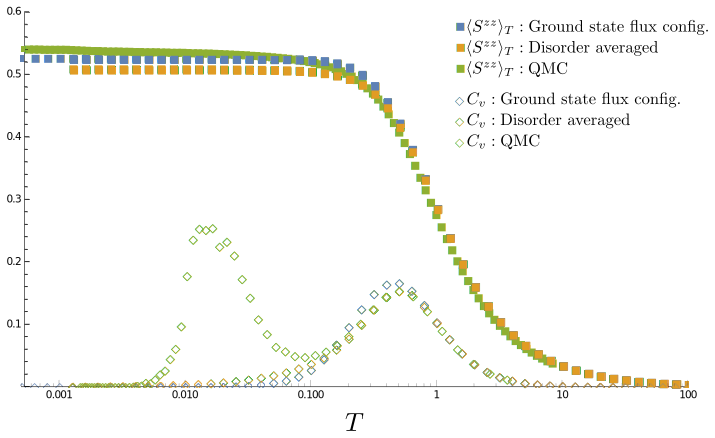
\includegraphics[width=0.8\linewidth]{./chapter07/HoneycombFiniteTempSpinSpinCorrelations.pdf}
	\caption{
		Nearest neighbor spin-spin correlations $S^{zz}$ and specific heat $C_v$ as a function of temperature for the Kitaev model on the honeycomb lattice.
		Comparison of a fixed ground state flux configuration (blue), averaging over random flux configurations (orange), and quantum Monte Carlo simulation (green).
	}
	\label{fig:chapter07_6_3SpinSpinCorrelations}
\end{figure}
%
To avoid explicitly performing the trace over all many-particle states, the above expressions are simplified as follows
(for notational simplicity, let $\Theta_\lambda = \beta \epsilon_\lambda/2$ and $\chi^{jk}_\mu = \psi^j_\mu \overline{\psi}^k_\mu$ in the following).
The fermionic partition function may be evaluated as
%
\begin{align}
	Z 	&= \sum_{\{n_\alpha\}_{\alpha=1}^N} \prod_{\lambda=1}^N \exp{\Big[(-1)^{n_\lambda} \Theta_\lambda\Big]} \nonumber\\
		&= \sum_{\{n_\alpha\}_{\alpha=2}^N} \sum_{n_1=0,1} \exp{[(-1)^{n_1} \Theta_1]} \prod_{\lambda=2}^N \exp{\Big[(-1)^{n_\lambda} \Theta_\lambda\Big]} \nonumber\\
%		&= 2\cosh{[\Theta_1]} \sum_{\{n_\alpha\}_{\alpha=2}^N} \prod_{\lambda=2}^N \exp{\Big[(-1)^{n_\lambda} \Theta_\lambda\Big]} \nonumber\\
		&= \prod_{\lambda=1}^N 2\cosh{[\Theta_\lambda]}.
\end{align}
%
The thermal Majorana two-point function can be simplified in an analogous manipulation as
%
\begin{align}
	\avg{\avg{c_j c_k}}_{T} &= \frac{1}{Z} \sum_{\{n_\alpha\}_{\alpha=1}^N} \avg{c_j c_k}_{\{n_\alpha\}} \exp{\Big[ -\beta \sum_{\lambda=1}^N \epsilon_\lambda (n_\lambda - 1/2) \Big]} \nonumber\\
							&= \frac{2}{Z} \sum_{\{n_\alpha\}_{\alpha=1}^N} \sum_{\mu=1}^N (-1)^{n_\mu} \chi^{jk}_\mu \prod_{\lambda=1}^N \exp{\Big[ (-1)^{n_\lambda} \Theta_\lambda \Big]} \nonumber\\
							&~~\vdots \nonumber\\
							&= \frac{2}{Z} \sum_{\mu=1}^N \chi^{jk}_\mu \tanh{[\Theta_\mu]} \prod_{\lambda=1}^N 2 \cosh{[\Theta_\lambda]} \nonumber\\
							&= 2 \sum_{\mu=1}^N \chi^{jk}_\mu \tanh{[\Theta_\mu]}.
\end{align}
Finally, the thermal spin-spin correlation function may be written in a fixed gauge as
\begin{align}
	\avg{S^{z z}}_T &= -\frac{i}{V} \sum_{\bR'} u_{AB}(\bR') \avg{\avg{c_A(\bR') c_B(\bR')}}_{T} \nonumber\\
					&= -\frac{2i}{V} \sum_{\bR'} u_{AB}(\bR') \sum_{\mu=1}^N \psi_\mu^A(\bR') \overline{\psi}_\mu^B(\bR') \tanh{[\beta \epsilon_\mu / 2]}.
	\label{eq:chapter07_ThermalSpinSpin}
\end{align}
%

Assuming a ground state gauge \textit{Ansatz}, the ground state expectation value is recovered as $T\rightarrow 0$.
Regardless of the gauge or flux configuration chosen, for $T\rightarrow \infty$ the spin-spin correlations vanish due to $\lim_{x\rightarrow 0} \left[\tanh{x}\right] = 0$.
For a more physical picture, recall from the last section that many-fermion states with complementary single-particle occupation numbers result in an equal but opposite contribution to a Majorana two-point function.
At high temperature where all states are weighted equally, contributions from such pairs of states will cancel each other, resulting in a vanishing of spin-spin correlations.
While the above analysis ignored thermal fluctuations of the gauge field by assuming a static configuration, the qualitative results are independent of this fact.
Moreover, for temperatures far enough above the gauge-field-disordering-crossover/transition, a simple averaging over random flux configurations may substitute the full-blown quantum Monte Carlo simulation.
%
\begin{figure}[tb]
	\centering
	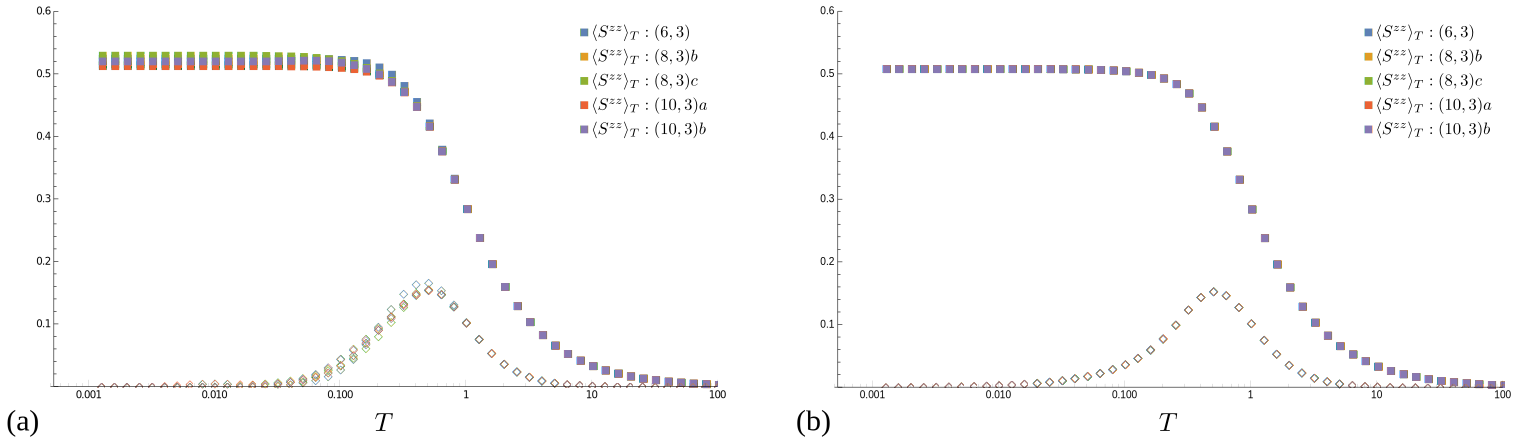
\includegraphics[width=\linewidth]{./chapter07/LatticesFiniteTempSpinSpinCorrelations.pdf}
	\caption{
		Nearest neighbor spin-spin correlations $S^{zz}$ and specific heat $C_v$ as a function of temperature for the Kitaev model on lattices (6,3), (8,3)b, (8,3)c, (10,3)a and (10,3)b.
		(a) Observables calculated in a fixed, ground state flux configuration.
		(b) Observables averaged over random flux configurations.
	}
	\label{fig:chapter07_LatticesSpinSpinCorrelations}
\end{figure}
%

In Figure~\ref{fig:chapter07_6_3SpinSpinCorrelations} are plotted three different data sets for the nearest-neighbor spin-spin correlation function $\avg{S^{zz}}_T$ and the specific heat $C_v$ for the honeycomb lattice as functions of temperature.
For the data set colored in blue, Eq.~\eqref{eq:chapter07_ThermalSpinSpin} was used to calculate the correlation function $\avg{S^{zz}}_T$ using a fixed gauge corresponding to the ground state flux configuration.
The specific heat was calculated directly from the single-particle spectrum.
The orange colored data set was similarly calculated from Eq.~\eqref{eq:chapter07_ThermalSpinSpin}, but this time the data was averaged over a large number of \textit{random} flux configurations.
Finally, the green data is taken from a quantum Monte Carlo simulation.

Although the correlations at very low temperature measured via quantum Monte Carlo are a little too large due to finite size effects, one can see from the figure that the data smoothly interpolates between the ground state flux sector data and the random flux sector data as temperature is increased.
Above the low-temperature crossover, the disorder-averaged data fits extremely well to the Monte Carlo simulation data.
In fact, the difference between the data calculated for the ground state flux sector differs very little from the disorder averaged data.
The disordering of the fluxes does not appear to shift the high-temperature crossover and, in general, only seems to suppress the value of the correlations slightly.
It was pointed out in Reference~\cite{NasuPRB2015} that as the fluxes become disordered, the linear scaling of the density of states near zero energy from the clean system is replaced by a finite density of states at zero energy. 
It may be that this large spectral weight at low energy is responsible for the suppression of correlations due to it being easier to excite many-fermion states at lower temperatures.

For a fixed density of \ZZ~fluxes -- whether that of the ground state flux sector or the maximally disordered flux configurations -- the spin-spin correlations are nearly constant up until the crossover temperature where excited many-fermion states destroy the correlations.
Coupled with the simultaneous release of fermionic entropy, this suggests that below the crossover temperature the only substantial contributions come from the fermionic ground state.

Finally, in Figure~\ref{fig:chapter07_LatticesSpinSpinCorrelations} are plotted the nearest neighbor spin-spin correlations $S^{zz}$ and specific heat $C_v$ as a function of temperature for the honeycomb lattice as well as a number of three-dimensional lattices -- both for a fixed ground state flux configuration and averaged over random flux configurations.
From Figure~\ref{fig:chapter07_LatticesSpinSpinCorrelations}~(a) the ground state value of the spin-spin correlations is seen to vary slightly from lattice to lattice, although the decay of correlations occurs at the same temperature.
However, when averaged over random flux configurations, the data is indistinguishable for the different lattices, as seen in Figure~\ref{fig:chapter07_LatticesSpinSpinCorrelations}~(b).
This is not so surprising as the low-energy density of states governing the low-temperature correlations for the disordered systems is in all cases governed by random matrix theory for the symmetry class BDI, and the center of mass of the single-particle density of states likely to control the position of the crossover is only slightly affected by disorder.
%
\begin{table}[tb]
	\centering
	\resizebox{\textwidth}{!}
	{\begin{tabular}{llrr}
		\hline
		\textbf{Lattice}             & \textbf{Gapless modes}	&	& \textbf{Exponent ($\alpha \approx d + d_c$)}     	\\ \hline
		\textbf{2D}                  & 							&	&							\\
		Square-octagon				 & Fermi line 				&	& 3.06 $\pm$ 0.08~~ 			$\approx~ 2 + 1$ \\
		Honeycomb					 & Dirac nodes        		&	& 3.995 $\pm$ 0.002~~ 		$\approx~ 2 + 2$ \\
		\textbf{3D}                  & 							&	&							\\
		(10,3)a 					 & Fermi surface     		&	& 3.93 $\pm$ 0.46~~ 			$\approx~ 3 + 1$ \\
		(10,3)b						 & Fermi line        		& In-plane:		& 5.15 $\pm$ 0.50~~	 $\approx~ 3 + 2$		\\
		& 							& Out-of-plane:	& 4.06 $\pm$ 0.01~~ 	 $\approx~ 4\;\,\phantom{+ 1}$			\\
		(10,3)c						 & Fermi line        		& In-plane: 	& 4.99 $\pm$ 0.30~~	 $\approx~ 3 + 2$		\\
		& 							& Out-of-plane:	& 3.96 $\pm$ 0.29~~	 $\approx~ 4\;\, \phantom{+ 1}$	 		\\
		(8,3)b 						 & Weyl nodes        		&	& 6.00 $\pm$ 0.06~~	 $\approx~ 3 + 3$ 		\\
	\end{tabular}}
	\caption{
		Overview of algebraic bond-bond correlations in gapless Kitaev spin liquids.
		The leading order long-wavelength behavior is seen to be given by $C(\br) \sim 1/\abs{\br}^{d + d_c}$, where $d$ is the spatial dimension and $d_c$ is the codimension of the nodal manifold.
	}
	\label{table:chapter07_BondBondCorrelations}
\end{table}
%
\newpage


%
%
%%%%%%%%%%%%%%%%%%%%%%%%%%%%%%%%%%%%%%%%%%%%%%%%%%%%%%%%%%%%%%%%%%%%%%%%%%%%%%%%%%%%%%%%
\section[Bond-bond correlations at zero temperature]{Bond-bond correlations at zero temperature}
\label{section:chapter07_BondBondCorrelationsZeroTemperature}
%%%%%%%%%%%%%%%%%%%%%%%%%%%%%%%%%%%%%%%%%%%%%%%%%%%%%%%%%%%%%%%%%%%%%%%%%%%%%%%%%%%%%%%%
%
%
%%%%%%%%%%%%%%%%%%%%%%%%%%%%%%%%%%%%%%%%%%%%%%%%%%%%%%%%%%%%%%%%%%%%%%%%%%%%%%%%%%%%%%%%
\subsection{General considerations and numerics}
\label{section:chapter07_BondBondGeneral}
%%%%%%%%%%%%%%%%%%%%%%%%%%%%%%%%%%%%%%%%%%%%%%%%%%%%%%%%%%%%%%%%%%%%%%%%%%%%%%%%%%%%%%%%
%
%
%%
%\begin{table}[tb]
%	\centering
%	\label{my-label}
%	\begin{tabular}{llrrr}
%		\hline
%		\textbf{Lattice}             & \textbf{Gapless modes}	&	& \textbf{Exponent ($\alpha \approx d + d_c$)}     	\\ \hline
%		\textbf{2D}                  & 							&	&							\\
%		Square-octagon				 & Fermi line 				&	& 3.06 $\pm$ 0.08~~ 			$\approx~ 3$	& $= 2 + 1$ \\
%		Honeycomb					 & Dirac nodes        		&	& 3.995 $\pm$ 0.002~~ 		$\approx~ 4$	& $= 2 + 2$ \\
%		\textbf{3D}                  & 							&	&							\\
%		(10,3)a 					 & Fermi surface     		&	& 3.93 $\pm$ 0.46~~ 			$\approx~ 4$	& $= 3 + 1$ \\
%		(10,3)b						 & Fermi line        		& In-plane:		& 5.15 $\pm$ 0.50~~	 $\approx~ 5$	& $= 3 + 2$		\\
%		& 							& Out-of-plane:	& 4.06 $\pm$ 0.01~~ 	 $\approx~ 4$	&		\\
%		(10,3)c						 & Fermi line        		& In-plane: 	& 4.99 $\pm$ 0.30~~	 $\approx~ 5$	& $= 3 + 2$		\\
%		& 							& Out-of-plane:	& 3.96 $\pm$ 0.29~~	 $\approx~ 4$	& 		\\
%		(8,3)b 						 & Weyl nodes        		&	& 6.00 $\pm$ 0.06~~	 $\approx~ 6$	& $= 3 + 3$ 		\\
%	\end{tabular}
%	\caption{
%		Overview of algebraic bond-bond correlations in gapless Kitaev spin liquids.
%		The leading order long-wavelength behavior is seen to be given by $C(\br) \sim 1/\abs{\br}^{d + d_c}$, where $d$ is the spatial dimension and $d_c$ is the codimension of the nodal manifold.
%	}
%	\label{table:chapter07_BondBondCorrelations}
%\end{table}
%%
In order to compute bond-bond correlations of the form
%
\begin{align}
	C(\bR) 	&= \frac{1}{V} \sum_{\bR'} \Big( \avg{\big(\sigma^z_A(\bR') \sigma^z_B(\bR')\big) \big(\sigma^z_A(\bR'+\bR) \sigma^z_B(\bR'+\bR)\big)}\nonumber\\
			&\qquad- \avg{\sigma^z_A(\bR') \sigma^z_B(\bR')} \avg{\sigma^z_A(\bR'+\bR) \sigma^z_B(\bR'+\bR)} \Big),
\end{align}
%
the spin operators should be expressed in the Majorana representation and the resulting Majorana four-point functions may be evaluated in terms of the Majorana two-point functions of the last section using Wick's theorem as
%
\begin{align}
	C(\bR) 	&= -\frac{4}{V} \sum_{\bR'} u_{AB}(\bR') u_{AB}(\bR' + \bR)~\times \nonumber\\
			&\qquad\sum_{\mu,\nu} \Bigg[\Big(\psi_{\mu}^A(\bR') \overline{\psi}_{\mu}^A(\bR' + \bR)\Big) \Big(\psi_{\nu}^B(\bR' + \bR) \overline{\psi}_{\nu}^B(\bR') \Big) \nonumber\\
			&\qquad\qquad+ \Big(\psi_{\mu}^A(\bR') \overline{\psi}_{\nu}^A(\bR' + \bR)\Big) \Big(\psi_{\nu}^B(\bR') \overline{\psi}_{\mu}^B(\bR' + \bR) \Big)\Bigg],
\end{align}
%
where the Greek indices are summed over single-particle states with non-negative energies as before.
For a translationally invariant system, \eg, at zero temperature, bond-bond correlations may be expressed particularly simply in terms of their Fourier components as
%
\begin{equation}
	C(\bR) = \frac{1}{\sqrt{V}} \sum_{\bk} e^{\-i \bk\cdot\bR} \tilde{C}(\bk)
	\label{eq:chapter07_BondBondInverseFourier}
\end{equation}
%
with
%
\begin{align}
	\tilde{C}(\bk) =	&-\frac{4}{V^{3/2}} \sum_{\bq} \sum_{\alpha,\beta} \Bigg[ \left|\psi_{\alpha}^A(\bk + \bq)\right|^2 \left|\psi_{\beta}^B(\bq)\right|^2 \nonumber\\
						&\qquad\qquad+ \left(\psi_{\alpha}^A(\bk + \bq) \overline{\psi}_{\beta}^A(\bq)\right) \left(\psi_{\beta}^B(\bq) \overline{\psi}_{\alpha}^B(\bk + \bq)\right) \Bigg],
	\label{eq:chapter07_BondBondZeroTFourier}
\end{align}
%
where the momenta are summed over the entire first Brillouin zone and $\alpha,\beta$ are band indices summed over non-negative energies at each momentum.

Eq.~\eqref{eq:chapter07_BondBondZeroTFourier} was used to numerically calculate bond-bond correlations in momentum space for the Kitaev model at the isotropic point ($J_x = J_y = J_z$) on a number of two- and three-dimensional lattices.
The real space data pictured in Figure~\ref{fig:chapter07_6_3BondBondPanel} was then arrived at by inverse Fourier transformation according to Eq.~\eqref{eq:chapter07_BondBondInverseFourier}.
While bond-bond correlations decay exponentially in the gapped spin liquid phases~\cite{YangPRA2008}, from Figure~\ref{fig:chapter07_6_3BondBondPanel} one may see that the gapless spin liquid phases exhibit algebraically decaying bond-bond correlations $C(\br) \sim 1/r^{\alpha}$, where the integer exponent $\alpha$ depends on the character of the gapless spin liquid.

The observation directions $\br$ shown in the plots of Figure~\ref{fig:chapter07_6_3BondBondPanel} were chosen to minimize the Friedel oscillations wherever possible.
The exponents $\alpha$ were found by fitting the log-log scaled data to a linear curve, ignoring the Friedel oscillations.
Table~\ref{table:chapter07_BondBondCorrelations} displays the different lattices along with the type of gapless modes it exhibits and the corresponding decay exponent $\alpha$.
Note that calculations for the square-octagon lattice are performed in the zero flux sector rather than in the ground state $\pi$-flux sector due to the ground state sector being gapless~\cite{YangPRB2007}.
From the data it can be seen that the decay exponent depends on both the dimension of the lattice \textit{and} the dimension of the nodal manifold.
Additionally, it can be seen in the case of Fermi lines in a three-dimensional Kitaev spin liquid that the value of the exponent depends on the observation direction $\br$.
While the power law fits to the data do not explain the presence of Friedel oscillations and yield approximately integer exponents, the next section provides a more detailed asymptotic analysis of the bond-bond correlation functions thereby demonstrating the origins of both.
%
\begin{figure}[p]
	\centering
	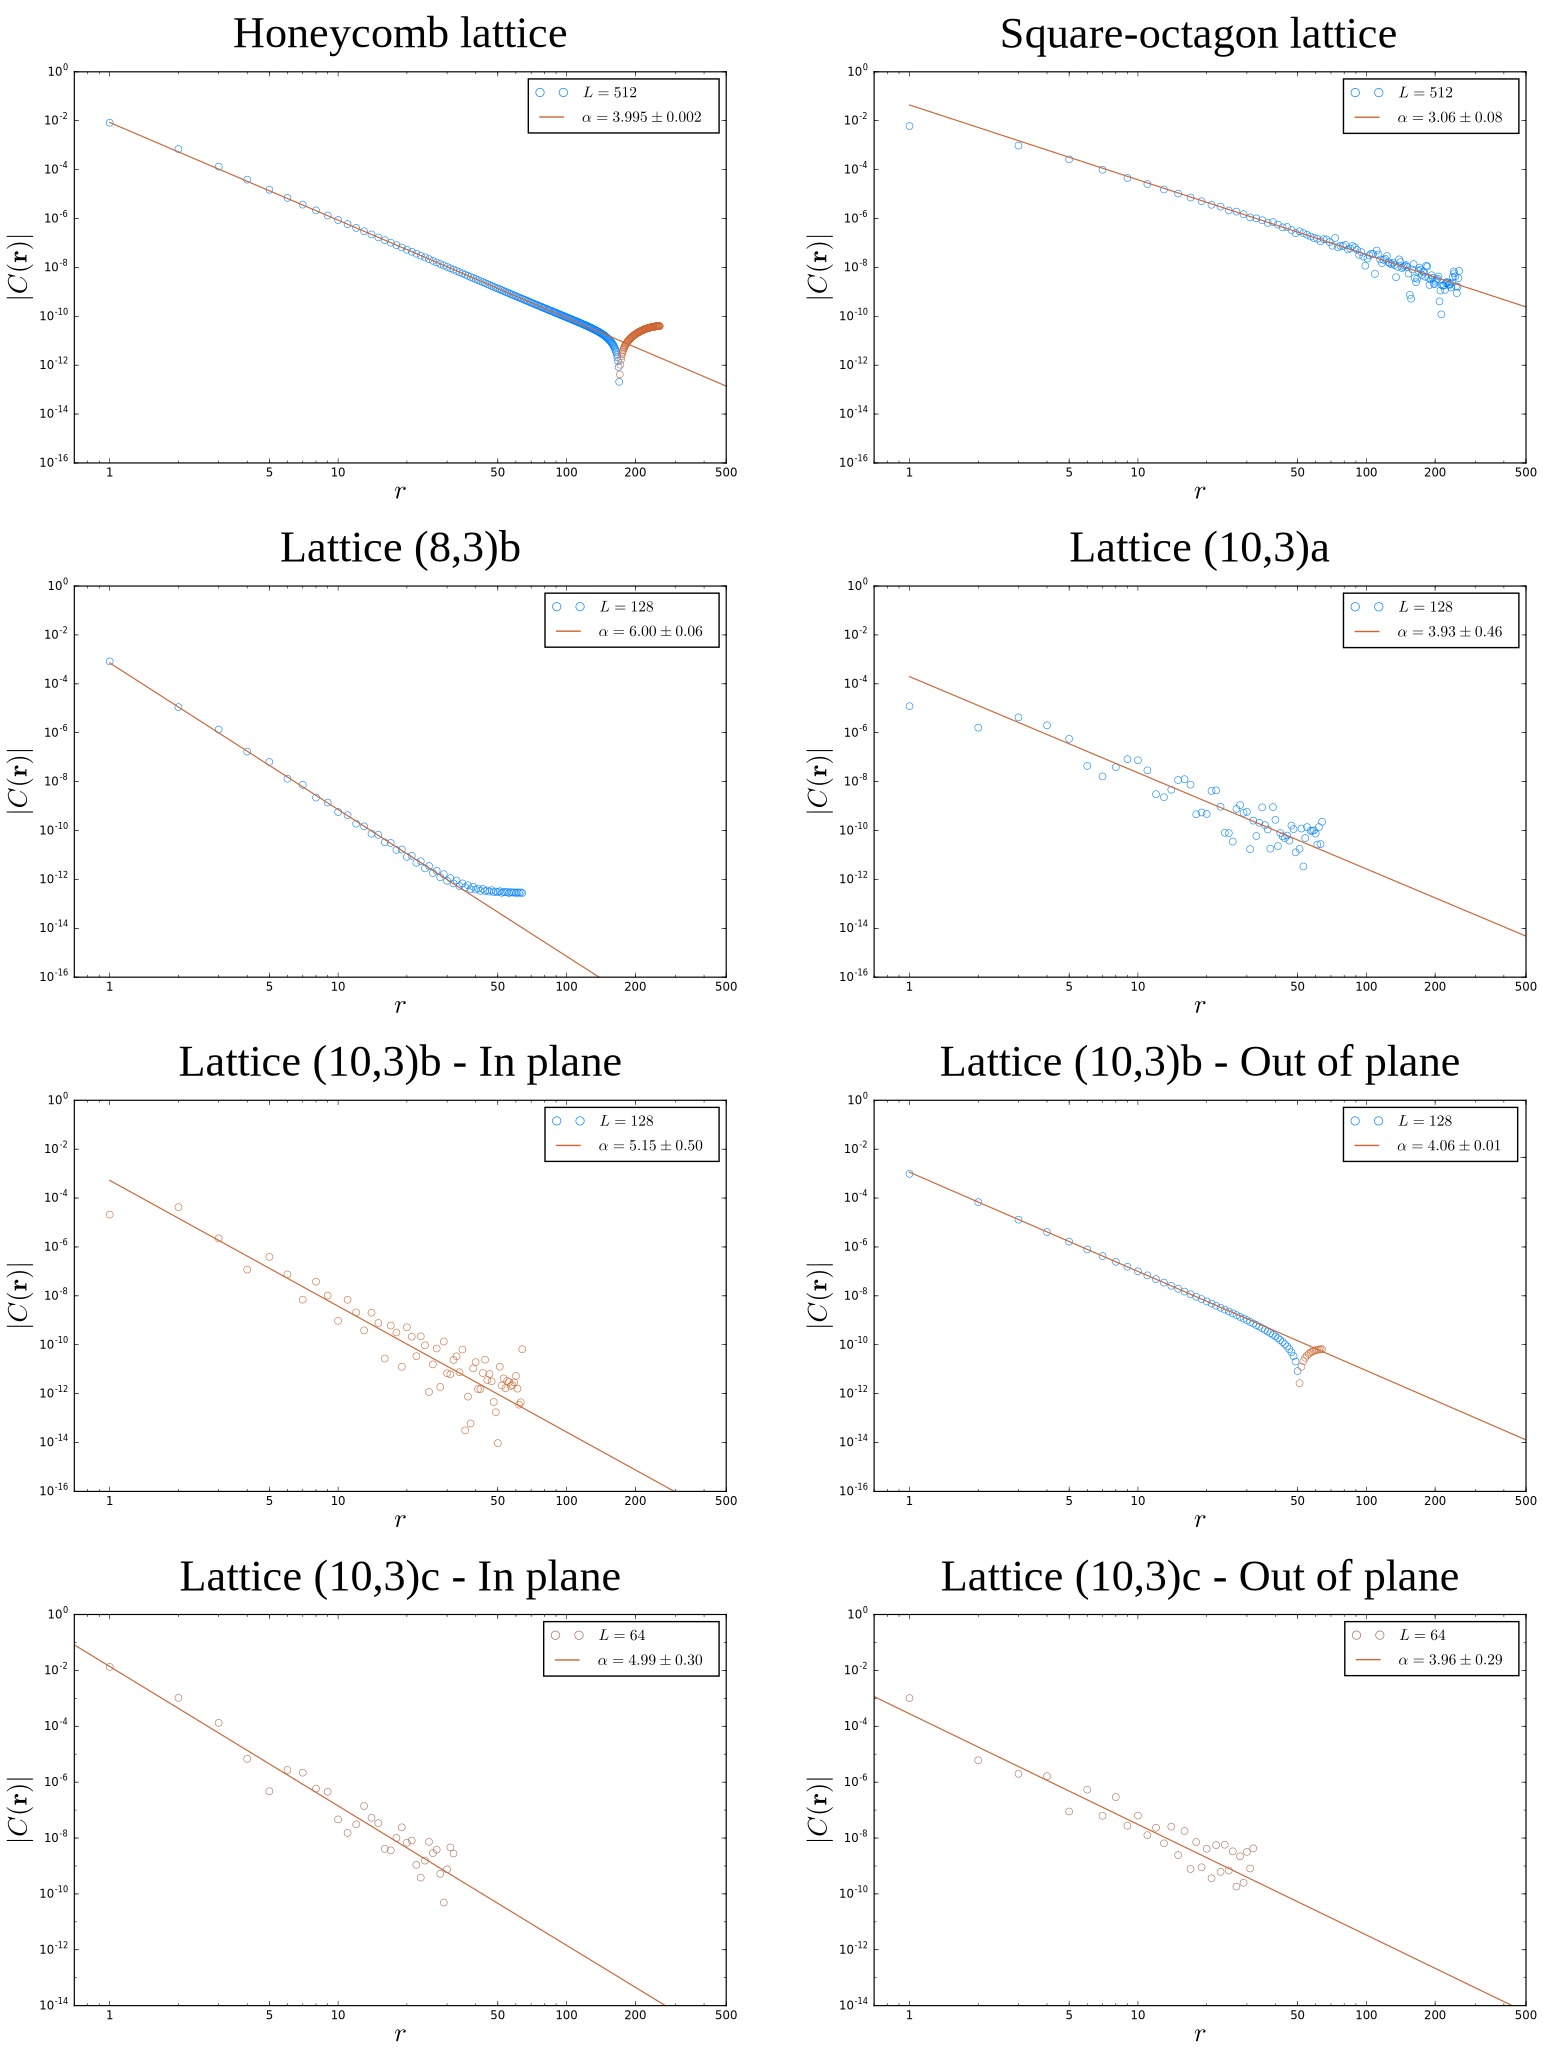
\includegraphics[width=\linewidth]{./chapter07/BondBondPanel.pdf}
	\caption{
		Bond-bond correlations $\abs{C(\br)}$ plotted on a log-log scale for gapless Kitaev spin liquids on a number of two- and three-dimensional lattices with $J_x = J_y = J_z$.
		Circles correspond to numerical data, whereas lines correspond to a linear fit through the data.
		The data is color coded blue and orange corresponding to positive and negative values of $C(\br)$, respectively.
		The two-dimensional honeycomb and square-octagon lattices host Dirac nodes and Fermi lines, respectively.
		The three-dimensional (8,3)b and (10,3)a lattices host Weyl nodes and Fermi surfaces, respectively, while lattices (10,3)b and (10,3)c host Fermi lines.
		Two directions are shown for lattices (10,3)b and (10,3)c corresponding to observation directions $\br$ both parallel (in plane) and perpendicular (out of plane) to the plane in which the Fermi line lies.
	}
	\label{fig:chapter07_6_3BondBondPanel}
\end{figure}
%


%
%
%%%%%%%%%%%%%%%%%%%%%%%%%%%%%%%%%%%%%%%%%%%%%%%%%%%%%%%%%%%%%%%%%%%%%%%%%%%%%%%%%%%%%%%%
\subsection{Asymptotic evaluation of correlation functions}
\label{section:chapter07_BondBondNumerics}
%%%%%%%%%%%%%%%%%%%%%%%%%%%%%%%%%%%%%%%%%%%%%%%%%%%%%%%%%%%%%%%%%%%%%%%%%%%%%%%%%%%%%%%%
%
%
In exploring the asymptotic behavior of the ground state bond-bond correlation functions, a translationally invariant gauge is assumed in order to yield
%
\begin{align}
	C(\br)	&= \avg{\sigma_A^z(\bz) \sigma_B^z(\bz) \sigma_A^z(\br) \sigma_B(\br)} - \avg{\sigma_A^z(\bz) \sigma_B^z(\bz)} \avg{\sigma_A^z(\br) \sigma_B^z(\br)} \nonumber\\
			&= \avg{c_A(\bz) c_A(\br)} \avg{c_B(\bz) c_B(\br)} - \avg{c_A(\bz) c_B(\br)} \avg{c_B(\bz) c_A(\br)}.
\end{align}
%
Whereas in previous sections creation operators $f\dag_{\alpha}$ were taken to correspond only to non-negative energy states, it is more convenient here to express the correlation functions in a way that allows the freedom to choose a specific polarization of creation and annihilation operators later, depending on the nature of the band structure at hand.
To this end, the Majorana two-point functions are expressed as
%
\begin{align}
	\avg{c_A(\bz) c_B(\br)} &= \frac{2}{V} \sum_{\alpha} \sum_{\bp} \Big[ e^{i \bp \cdot \br} \psi_{\alpha}^A(\bp) \bar{\psi}_{\alpha}^B(\bp) \avg{f_{\alpha, \bp} f\dag_{\alpha, \bp}} \nonumber\\
							&\qquad\qquad\qquad+ e^{-i \bp \cdot \br} \psi_{\alpha}^B(\bp) \bar{\psi}_{\alpha}^A(\bp) \avg{f\dag_{\alpha, \bp} f_{\alpha, \bp}} \Big],
\end{align}
%
where $\psi_{\alpha}(\bp)$ is a complex wave function of band $\alpha$ with momentum $\bp$ which is summed over the entire first Brillouin zone.
Given that there are $2n$ sites in a unit cell, the $\alpha$ summation is over $n$ energy bands.
Substituting this into the expression for the bond-bond correlations and defining $\chi_{\alpha}^{AB}(\bp) = \psi_{\alpha}^A(\bp) \overline{\psi}_{\alpha}^B(\bp) = \overline{\chi}_{\alpha}^{BA}(\bp)$ for notational convenience,
%
\begin{align}
	C(\br)	&= \frac{4}{V^2} \sum_{\alpha, \beta} \sum_{\bp, \bq} \Bigg[ \Bigg(e^{i (\bp + \bq) \cdot \br} \chi_{\alpha}^{AA}(\bp) \chi_{\beta}^{BB}(\bq) \avg{f_{\alpha, \bp} f\dag_{\alpha, \bp}} \avg{f_{\beta, \bq} f\dag_{\beta, \bq}} \nonumber \\
			&\qquad+ e^{i (\bp - \bq) \cdot \br} \chi_{\alpha}^{AA}(\bp) \chi_{\beta}^{BB}(\bq) \avg{f_{\alpha, \bp} f\dag_{\alpha, \bp}} \avg{f\dag_{\beta, \bq} f_{\beta, \bq}} + h.c. \Bigg) \nonumber \\
			&\qquad- \Bigg(e^{i (\bp + \bq) \cdot \br} \chi_{\alpha}^{AB}(\bp) \chi_{\beta}^{BA}(\bq) \avg{f_{\alpha, \bp} f\dag_{\alpha, \bp}} \avg{f_{\beta, \bq} f\dag_{\beta, \bq}} \nonumber \\
			&\qquad+ e^{i (\bp - \bq) \cdot \br} \chi_{\alpha}^{AB}(\bp) \chi_{\beta}^{AB}(\bq) \avg{f_{\alpha, \bp} f\dag_{\alpha, \bp}} \avg{f\dag_{\beta, \bq} f_{\beta, \bq}} + h.c. \Bigg) \Bigg].
	\label{eq:chapter07_BondBondFull}
\end{align}
%

In the following, only the asymptotic behavior of Eq.~\eqref{eq:chapter07_BondBondFull} will be of interest and a few approximations may be made.
Terms such as
%
\begin{equation}
	\sum_{\alpha} \sum_{\bp} e^{i \bp \cdot \br} \chi_{\alpha}^{AA}(\bp) \avg{f_{\alpha, \bp} f\dag_{\alpha, \bp}} 
\end{equation}
%
are replaced by
%
\begin{equation}
	\frac{V}{(2\pi)^D} \sum_{\bp^*} e^{i \bp^* \cdot \br} \int d\bp~e^{i \bp \cdot \br} \chi_{FS}^{AA}(\bp^* + \bp) \avg{f_{FS}(\bp^* + \bp) f\dag_{FS}(\bp^* + \bp)},
	\label{eq:chapter07_TwoPointAsymptotic}
\end{equation}
%
where $\bp^*$ are the points on the nodal manifold at which $\br$ is orthogonal to the tangent to the nodal manifold and $\bp$ is the momentum relative to that point.
For point nodes, $\bp^*$ is just the position of the node regardless of the choice of $\br$.
Only the band $\alpha \equiv FS$ which crosses the Fermi energy is considered.
Finally, the wave functions and fermion Green's functions are evaluated using a low-energy approximation near the respective points $\bp^*$.
Terms similar in form are evaluated analogously.
From Eq.~\eqref{eq:chapter07_TwoPointAsymptotic} it can be seen that the points $\bp^*, \bq^*$ determine the wavevectors of the Friedel oscillations, whereas the approximate low-energy wave functions and fermion Green's functions determine how these oscillations decay.
The rest of this section is dedicated to a detailed analysis of the asymptotic bond-bond correlation function for the two-dimensional honeycomb and square-octagon lattices.
After the basic machinery is introduced for these two cases, some remarks about the remaining three-dimensional lattices are made.


%
%
%%%%%%%%%%%%%%%%%%%%%%%%%%%%%%%%%%%%%%%%%%%%%%%%%%%%%%%%%%%%%%%%%%%%%%%%%%%%%%%%%%%%%%%%
\subsubsection{Square-octagon lattice}
\label{section:chapter07_BondBondSquareOctagon}
%%%%%%%%%%%%%%%%%%%%%%%%%%%%%%%%%%%%%%%%%%%%%%%%%%%%%%%%%%%%%%%%%%%%%%%%%%%%%%%%%%%%%%%%
%
%
Working in the zero-flux sector, the two-dimensional square-octagon lattice hosts a pair of nodal lines separated by a perfect nesting vector $\bk_0 = (\bq_1 + \bq_2)/2$ due to a non-trivially implemented projective time-reversal operator, where $\bq_1, \bq_2$ are the reciprocal lattice vectors for the lattice.
The gapless band structure along with the nodal lines at the isotropic point are pictured in Figure~\ref{fig:chapter07_SquareOctagonPanel1}.
In the following, only the bands which cross the Fermi level are of concern.
In fact, here will be used the convention that the fermionic creation operators $f\dag$ correspond to the band which is colored blue in Figure~\ref{fig:chapter07_SquareOctagonPanel1}~(a) which generates the blue Fermi line in Figure~\ref{fig:chapter07_SquareOctagonPanel1}~(b).
By particle-hole symmetry, the analogous annihilation operators correspond to the orange colored band.
Therefore, in this picture there is only a single nodal line.
%
\begin{figure}[tb]
	\centering
	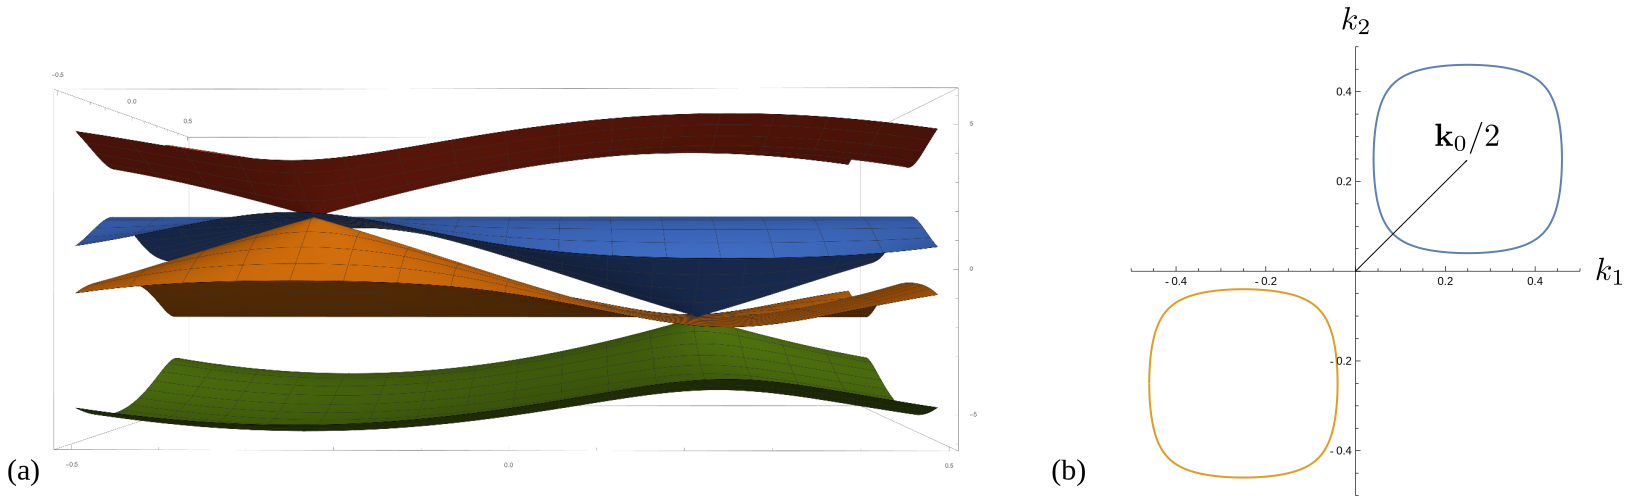
\includegraphics[width=\linewidth]{./chapter07/SquareOctagonPanel1.pdf}
	\caption{
		(a) Gapless band structure of the Kitaev model on the square-octagon lattice.
		(b) Nodal lines of the Kitaev model on the square-octagon lattice.
	}
	\label{fig:chapter07_SquareOctagonPanel1}
\end{figure}
%

There are essentially two types of terms to calculate: those for which both fermions come from either above or below the Fermi level (referred to below as particle-particle or hole-hole terms, respectively), \ie,
%
\begin{equation}
	\propto e^{i (\bp^* + \bq^*) \cdot \br} \avg{f_{FS}(\bp^* + \bp) f\dag_{FS}(\bp^* + \bp)} \avg{f_{FS}(\bq^* + \bq) f\dag_{FS}(\bq^* + \bq)},
\end{equation}
%
and those for which one fermion comes from above (below) the Fermi level while the other comes from below (above) the Fermi level (referred to below as particle-hole or hole-particle terms, respectively), \ie,
%
\begin{equation}
	\propto e^{i (\bp^* - \bq^*) \cdot \br} \avg{f_{FS}(\bp^* + \bp) f\dag_{FS}(\bp^* + \bp)} \avg{f\dag_{FS}(\bq^* + \bq) f_{FS}(\bq^* + \bq)}.
\end{equation}
%

For the determination of Friedel oscillations one additionally needs the values of $\bp^*$ and $\bq^*$.
The first case to consider is $\bp^* = \bq^*$.
For particle-hole terms which have prefactor $e^{i(\bp^* - \bq^*)\cdot\br}$, there are no oscillations.
However, particle-particle terms which have prefactor $e^{i(\bp^* + \bq^*)\cdot\br}$ generate oscillations with wavevector $\bk = 2\bk_F(\bp^*) + \bk_0$, where $\bk_F(\bp^*) = \bp^* - \bk_0/2$ (refer to Figure~\ref{fig:chapter07_SquareOctagonPanel1}~(b)).
Friedel oscillations for hole-particle or hole-hole terms are determined in the same manner.

Next consider the role of time-reversal symmetry which maps $\bq \mapsto -\bq + \bk_0$ and take $\bp^*, \bq^*$ to be time-reversal pairs, \ie, $\bq^* = -\bp^* + \bk_0$.
For particle-hole terms which have prefactor $e^{i(\bp^* - \bq^*)\cdot\br}$, there will be oscillations with wavevector $\bk = 2\bk_F(\bp^*)$.
Particle-particle terms which have prefactor $e^{i(\bp^* + \bq^*)\cdot\br}$ generate oscillations with wavevector $\bk = \bk_0$.
Again, the Friedel oscillations for hole-particle or hole-hole terms are determined in the same manner.

At these wavevectors one can expect singular behavior in the Fourier transform of the bond-bond correlation function resulting in an algebraic decay in real space.
In order to determine the manner in which the correlation function decays, one must calculate the asymptotic behavior of the integrals of Eq.~\eqref{eq:chapter07_TwoPointAsymptotic}.
Since the wave function terms $\chi_{FS}$ are smooth and non-vanishing at the Fermi level, they will be approximated as constants and replaced by their value at the corresponding points $\bp^*, \bq^*$.
The long distance behavior then comes from the sharp cutoff of the Green's functions at the Fermi level.

To calculate this, the quasiparticle energy is expanded about the points $\bp^*, \bq^*$ as, \eg,
%
\begin{equation}
	\epsilon(\bp^* + \bp) = v_F \left( \zeta p_{\parallel} + \frac{\alpha}{2} p_{\bot}^2 \right),
\end{equation}
%
where $p_{\parallel}$ and $p_{\bot}$ are the components of $\bp$ parallel and perpendicular to $\br$, respectively, $v_F$ and $\alpha$ are the Fermi velocity and curvature of the Fermi surface at the point $\bp^*$, respectively, and $\zeta = \pm 1$ depending on whether the fermion is right or left moving at the point $\bp^*$.
Using this approximation, the real-space Green's functions may be calculated, \eg, for a right-moving fermion as
%
\begin{align}
	&\int d^2p~ e^{i\bp\cdot\br} \avg{f_{FS}(\bp) f\dag_{FS}(\bp)} = \int dp_{\parallel} e^{i p_{\parallel} r} \int dp_{\bot}~ H(\epsilon(\bp^* + \bp)) \nonumber\\
	&\qquad\approx \int_{-\infty}^{\infty} dp_{\parallel} e^{i p_{\parallel} r} H(-p_{\parallel})\Bigg[\int_{-\Lambda}^{-\sqrt{-2p_{\parallel}/\alpha}} dp_{\bot} + \int_{\sqrt{-2p_{\parallel}/\alpha}}^{\Lambda} dp_{\bot}\Bigg] \nonumber\\
	&\qquad\qquad+ \int_{-\infty}^{\infty} dp_{\parallel}~ e^{i p_{\parallel} r} H(p_{\parallel}) \int_{-\Lambda}^{\Lambda} dp_{\bot},
\end{align}
%
where $H(x)$ is the Heaviside step function and $\Lambda$ is an arbitrary momentum cutoff which does not affect the final result.
Only the first two terms contribute to the long-wavelength behavior of the correlation function and may be evaluated as~\cite{Lighthill1958}
%
\begin{align}
	\int d^2p~ e^{i\bp\cdot\br} \avg{f_{FS}(\bp) f\dag_{FS}(\bp)} &\approx -2\sqrt{\frac{2}{\alpha}} \int_{-\infty}^{\infty} dp_{\parallel} e^{i p_{\parallel} r} \abs{p_{\parallel}}^{1/2} H(-p_{\parallel}) \nonumber\\
	&= -\sqrt{\frac{2\pi}{\alpha}} \frac{e^{-i 3\pi/4}}{r^{3/2}}.
\end{align}
%
The remainder of the real-space Green's functions may be evaluated similarly yielding
%
\begin{align}
	\int d^2p~ e^{i\bp\cdot\br} \avg{f_{FS}(\bp) f\dag_{FS}(\bp)} &\approx -\sqrt{\frac{2\pi}{\alpha}} \frac{e^{-\zeta i 3\pi/4}}{r^{3/2}} \nonumber\\
	\int d^2p~ e^{-i\bp\cdot\br} \avg{f\dag_{FS}(\bp) f_{FS}(\bp)} &\approx \sqrt{\frac{2\pi}{\alpha}} \frac{e^{\zeta i 3\pi/4}}{r^{3/2}},
\end{align}
%
where $\zeta = \pm 1$ for $\bp^*$ corresponding to right- and left-moving fermions, respectively.
%
\begin{figure}[tb]
	\centering
	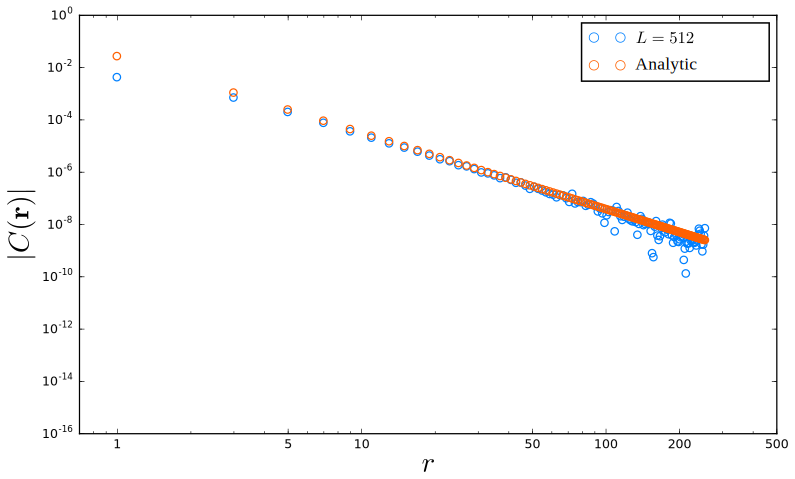
\includegraphics[width=0.8\linewidth]{./chapter07/SquareOctagonPanel2.pdf}
	\caption{
		Comparison of numerics and analytics for bond-bond correlations on the square-octagon lattice for $\br = r \ba_1$.
	}
	\label{fig:chapter07_SquareOctagonPanel2}
\end{figure}
%

The final analytic expression for the bond-bond correlation function must contain terms from all combinations of $\bp^*$ and $\bq^*$ and is rather lengthy, however, it can already be seen from here that the correlations will decay as a power law $C(\br) \sim 1/r^3$.
Using numerically obtained values for $\alpha$, $\bp^*$, $\bq^*$ and the wave functions, Figure~\ref{fig:chapter07_SquareOctagonPanel2} shows a comparison of the asymptotic expression derived above to the numerically obtained data discussed in Section~\ref{section:chapter07_BondBondGeneral} for $\br = r \ba_1$, where $\ba_1$ is a lattice vector of the square-octagon lattice.
Other than finite size effects for larger values of $r$, the asymptotic expression yields a very good fit to the data.
One can see in the figure that bond-bond correlations vanish entirely for even values of $r$ due to the perfect nesting vector $\bk_0$, as the bond-bond correlation function in the $\ba_1$-direction takes the general form
%
\begin{equation}
	C(\br) \propto \frac{1 - \cos{(\bk_0 \cdot \br)}}{r^3} = \frac{1 - \cos{(\pi r)}}{r^3}.
\end{equation}
%


%
%
%%%%%%%%%%%%%%%%%%%%%%%%%%%%%%%%%%%%%%%%%%%%%%%%%%%%%%%%%%%%%%%%%%%%%%%%%%%%%%%%%%%%%%%%
\subsubsection{Honeycomb lattice}
\label{section:chapter07_BondBondHoneycomb}
%%%%%%%%%%%%%%%%%%%%%%%%%%%%%%%%%%%%%%%%%%%%%%%%%%%%%%%%%%%%%%%%%%%%%%%%%%%%%%%%%%%%%%%%
%
%
As already mentioned in this thesis, the gapless Kitaev spin liquid on the honeycomb lattice hosts two Dirac nodes corresponding to two linearly-dispersing bands as pictured in Figure~\ref{fig:chapter07_HoneycombDispersion}.
In the following, the convention is used such that fermionic creation operators $f\dag$ correspond to the band which is colored blue in the figure.
This band touches the Fermi level at two Dirac nodes located at $\pm \bk_{\rm Dirac} = \pm (\bq_1 - \bq_2)/3$.
As all states lie below the Fermi level, the only non-vanishing terms contributing to the bond-bond correlation functions are the hole-hole terms, \ie,
%
\begin{equation}
	\propto e^{-i (\bp^* + \bq^*) \cdot \br} \avg{f\dag_{FS}(\bp^* + \bp) f_{FS}(\bp^* + \bp)} \avg{f\dag_{FS}(\bq^* + \bq) f_{FS}(\bq^* + \bq)}.
\end{equation}
%
%
\begin{figure}[tb]
	\centering
	\includegraphics[width=0.9\linewidth]{./chapter07/HoneycombDispersion.pdf}
	\caption{
		Gapless Dirac cone band structure of the Kitaev model on the honeycomb lattice.
	}
	\label{fig:chapter07_HoneycombDispersion}
\end{figure}
%

For the determination of Friedel oscillations one additionally needs the values of $\bp^*$ and $\bq^*$.
For the honeycomb lattice there are only two such points, \ie, the locations of the Dirac nodes.
The first case to consider is $\bp^* = \bq^*$.
Hole-hole terms which have prefactor $e^{-i(\bp^* + \bq^*)\cdot\br}$ will generate oscillations with wavevector $\bk = \pm 2\bk_{\rm Dirac}$.
Next, consider the role of time-reversal symmetry which maps $\bq \mapsto -\bq$.
For time-reversal pairs $\bq^* = -\bp^*$, hole-hole terms with prefactor $e^{-i(\bp^* + \bq^*)\cdot\br}$ do not result in Friedel oscillations, \ie, $\bk = \bz$.

At these wavevectors one can expect singular behavior in the Fourier transform of the bond-bond correlation function resulting in an algebraic decay in real space.
The Green's functions are equal to unity for all momenta due to the semi-metallic nature of the fermion dispersion, therefore, the algebraic correlations come from the non-analyticity of the wave functions at the Dirac nodes.
Terms such as $\chi_{FS}^{AA}$ and $\chi_{FS}^{BB}$ are constant for all momenta and, thus, do not contribute to the long-wavelength behavior of the correlation function.
In this case, the relevant expression for the asymptotic bond-bond correlation function is given by
%
\begin{equation}
	C(\br) \sim -\frac{4}{(2\pi)^4} \sum_{\bp^*, \bq^*} e^{-i(\bp^* + \bq^*)\cdot\br} \int d^2p~d^2q~ e^{-i(\bp + \bq)\cdot\br} \chi_{FS}^{AB}(\bp^* + \bp) \chi_{FS}^{BA}(\bq^* + \bq).
\end{equation}
%
Setting $J_x = J_y = (1 - J_z)/2$, expanding the wave functions about the Dirac nodes and summing over $\bp^*$ and $\bq^*$, one arrives at an expression for the correlation function
%
\begin{align}
	C(\br) &\sim -\frac{4}{(2\pi)^4} \int d^2p~d^2q~ e^{-i(\bp + \bq)\cdot\br}~\times \nonumber\\
	&\qquad\Bigg\{ 2\cos{(2\bk_{\rm Dirac}\cdot\br)}\left[A^2 - B^2 + C^2 - D^2 + 2CE + E^2 - 2DF - F^2\right] \nonumber\\
	&\qquad\phantom{\Bigg\{}+ 4i\sin{(2\bk_{\rm Dirac}\cdot\br)}\left[-AC + BD - AE + BF\right] \nonumber\\
	&\qquad\phantom{\Bigg\{}+ 2\left[A^2 + B^2 - C^2 - D^2 - 2CE - E^2 - 2DF - F^2\right]\Bigg\},
\end{align}
%
where
%
\begin{equation}
	\begin{matrix*}[l]
		A = -\dfrac{v_y p_y}{2\sqrt{v_x^2 p_x^2 + v_y^2 p_y^2}}, &
		B = i\dfrac{v_x p_x}{2\sqrt{v_x^2 p_x^2 + v_y^2 p_y^2}}, \\
		&\\
		C = -\dfrac{3 \alpha J_z v_x^3 v_y p_x^3 p_y}{8(v_x^2 p_x^2 + v_y^2 p_y^2)^{3/2}}, &
		D = -i\dfrac{3 \alpha J_z v_x^2 v_y^2 p_x^2 p_y^2}{8(v_x^2 p_x^2 + v_y^2 p_y^2)^{3/2}}, \\
		&\\
		E = -\dfrac{v_x v_y^3 p_x p_y^3}{8 J_z (v_x^2 p_x^2 + v_y^2 p_y^2)^{3/2}}, &
		F = -i\dfrac{v_y^4 p_y^4}{8 J_z (v_x^2 p_x^2 + v_y^2 p_y^2)^{3/2}},
	\end{matrix*}
\end{equation}
%
and with
%
\begin{equation}
	\begin{matrix*}[l]
		v_x = \sqrt{1 - 2J_z},	& \qquad\qquad	& v_y = \sqrt{3} J_z,	\\
		\\
		\alpha = J_z \left(\frac{1}{3 v_x^2} + \frac{2}{v_y^2}\right),	& \qquad\qquad	& \bk_{\rm Dirac} = \frac{1}{2\pi} \arccos{\left(-\frac{J_z}{1 - J_z}\right)} (\bq_1 - \bq_2).
	\end{matrix*}
\end{equation}
%

One may now choose a direction for $\br$ and evaluate the integrals analogously to what was done for the square-octagon lattice above~\cite{Lighthill1958}.
For $\br = r(\ba_1 + \ba_2)$ there are no Friedel oscillations due to $2\bk_{\rm Dirac}\cdot\br = 0$.
The bond-bond correlations for the $(\ba_1 + \ba_2)$-direction may be evaluated as
%
\begin{equation}
	C(\br) \sim \frac{v_y^2}{v_x^2}\frac{1}{9\pi^2 r^4}.
\end{equation}
%
Comparing to the numerical data in Figure~\ref{fig:chapter07_HoneycombPanel}, the asymptotic expression above provides a good fit, reproducing the $1/r^4$ behavior seen in Section~\ref{section:chapter07_BondBondGeneral}.
As the exchange couplings are tuned within the gapless phase, only the overall prefactor of the correlations changes.

The bond-bond correlations are more complicated for $\br = r(\ba_1 - \ba_2)$.
In this case the correlation function may be evaluated as
%
\begin{align}
	C(\br) \sim &-\frac{v_x^2}{2\pi^2 v_y^2} \left[1 - \cos{(2\bk_{\rm Dirac}\cdot\br)}\right] \frac{1}{r^4} \nonumber\\
	&-\frac{3 v_x^3 (1 - 2\alpha J_z)}{4\pi^2 J_z v_y^2} \sin{(2\bk_{\rm Dirac}\cdot\br)} \frac{1}{r^5} \nonumber\\
	&-\frac{9 v_x^4 (1 - 2\alpha J_z)^2}{32 \pi^2 J_z^2 v_y^2} \left[1 + \cos{(2\bk_{\rm Dirac}\cdot\br)}\right] \frac{1}{r^6}.
\end{align}
%
Comparing to the numerical data in Figure~\ref{fig:chapter07_HoneycombPanel}, the asymptotic expression above provides a good fit.
At the isotropic point one sees that the $1/r^4$ term dominates for $r \neq 0~({\rm mod}~3)$, whereas the $1/r^6$ term dominates for $r = 0~({\rm mod}~3)$ due to an exact cancellation of the leading order term from Friedel oscillations.
Away from the isotropic point where $2\bk_{\rm Dirac}\cdot\br \neq 0~({\rm mod}~2\pi)$ for integer $r$, there is a complex interplay of all three terms.
Using the asymptotic analysis here, even this more complex behavior is captured.
%
\begin{figure}[tb]
	\centering
	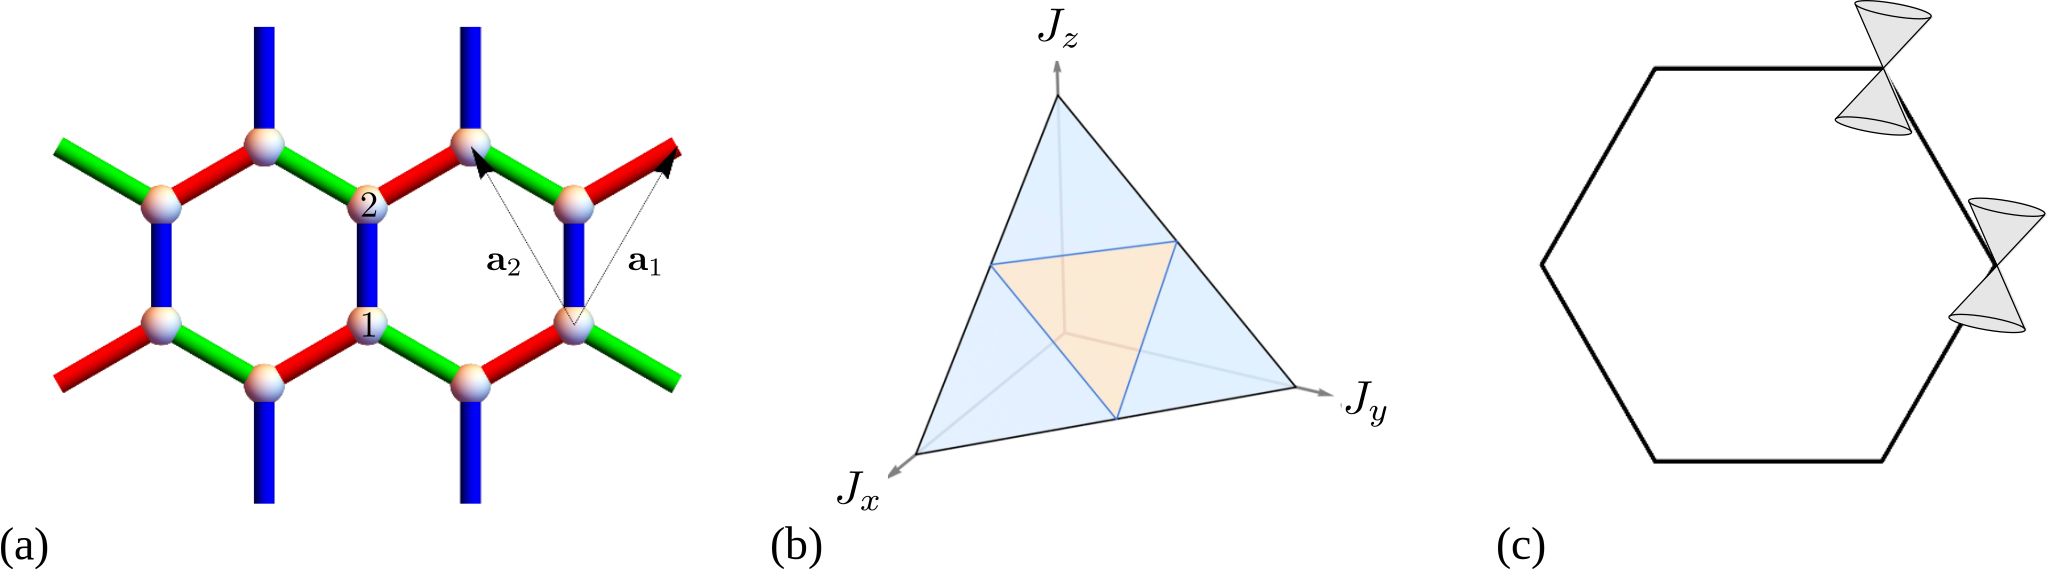
\includegraphics[width=\linewidth]{./chapter07/HoneycombPanel.pdf}
	\caption{
		Comparison of numerics and analytics for bond-bond correlations on the honeycomb lattice for (left) $\br = r (\ba_1 + \ba_2)$ and (right) $\br = r (\ba_1 - \ba_2)$ with $J_x = J_y = (1 - J_z)/2$ for (top) $J_z > J_x, J_y$, (middle) $J_z = J_x = J_y$ and (bottom) $J_z < J_x, J_y$.
	}
	\label{fig:chapter07_HoneycombPanel}
\end{figure}
%


%
%
%%%%%%%%%%%%%%%%%%%%%%%%%%%%%%%%%%%%%%%%%%%%%%%%%%%%%%%%%%%%%%%%%%%%%%%%%%%%%%%%%%%%%%%%
\subsubsection{Three-dimensional lattices}
\label{section:chapter07_BondBondThreeDimensions}
%%%%%%%%%%%%%%%%%%%%%%%%%%%%%%%%%%%%%%%%%%%%%%%%%%%%%%%%%%%%%%%%%%%%%%%%%%%%%%%%%%%%%%%%
%
%
While a thorough investigation of the asymptotic behavior of the bond-bond correlation function has not been performed for the three-dimensional lattices, some general remarks may be made.
The simplest case to study is for fully two-dimensional Fermi surfaces as in lattice (10,3)a.
Similar to the nodal line in \textit{two}-dimensions, the algebraic decay comes from the sharp cutoff of the momentum-space fermion Green's functions at the Fermi level.
For the Fermi surface in three-dimensions, the fermion Green's functions take the form~\cite{Lighthill1958}, \eg,
%
\begin{align}
	\int d^3p~ e^{i\bp\cdot\br} \avg{f_{FS}(\bp) f\dag_{FS}(\bp)} &\sim \frac{2}{\sqrt{\alpha}} \int_{-\infty}^{\infty} dp_{\parallel}~ e^{i p_{\parallel} r} \abs{p_{\parallel}} H(-p_{\parallel}) \nonumber\\
	&\sim \frac{1}{r^2},
\end{align}
%
yielding a bond-bond correlation function which decays as $C(\br) \sim 1/r^4$, as is seen in the numerical data of Section~\ref{section:chapter07_BondBondGeneral}.

The semi-metallic cases of Fermi lines and Weyl nodes in three-dimensions are more complicated as the algebraic correlations come from the non-analyticity of the fermion wave functions rather than from the Green's functions.
As one does not have access to an analytic expression for the wave functions here as opposed to the case of the two-dimensional Dirac nodes, one must resort to idealized wave functions for the two cases.
This analysis has not been performed, but some general remarks and speculation will be made.

For the Fermi line in three-dimensions, one might assume a wave function of the same form as the Dirac nodes in the last section, where $p_x$ and $p_y$ now correspond to two directions orthogonal to the Fermi line.
For the direction tangent to the Fermi line, the wave function should be well-behaved and not contribute anything additional to the long-wavelength behavior of the correlation functions.
In this idealized case, one would expect correlations to decay as $C(\br) \sim 1/r^4$ just as for the Dirac nodes in two-dimensions.
For observation directions $\br$ \textit{orthogonal} to the plane in which the Fermi line lies and where all points on the Fermi line contribute, this is indeed the behavior seen in the numerics presented in Section~\ref{section:chapter07_BondBondGeneral}.
The author speculates that for the observation directions $\br$ \textit{parallel} to the plane in which the Fermi line lies, the observed $1/r^5$ decay is due to a cancellation of the leading order $1/r^4$ term similar to what was seen to occur for the Dirac nodes.

Finally, the author has not performed an analysis for the case of the Weyl nodes in three-dimensions, but imagines that the calculation of the decay envelope may be performed straightforwardly by assuming an idealized wave function for a Weyl node similar to what was described for the Fermi line above.


%
%
%%%%%%%%%%%%%%%%%%%%%%%%%%%%%%%%%%%%%%%%%%%%%%%%%%%%%%%%%%%%%%%%%%%%%%%%%%%%%%%%%%%%%%%%
\section{Bond-bond correlations at finite temperature}
\label{section:chapter07_BondBondCorrelationsFiniteTemperature}
%%%%%%%%%%%%%%%%%%%%%%%%%%%%%%%%%%%%%%%%%%%%%%%%%%%%%%%%%%%%%%%%%%%%%%%%%%%%%%%%%%%%%%%%
%
%
As was done for the nearest-neighbor spin-spin correlations in Section~\ref{section:chapter07_SpinSpinCorrelationsFiniteTemperature}, one may similarly ask what is the fate of the bond-bond correlation function at finite temperature.
In order to calculate the thermal bond-bond correlation function, one needs to evaluate thermal expectation values of products of Majorana two-point functions of the form
%
\begin{equation}
	\avg{\avg{c_i c_j}\avg{c_k c_l}}_{T} = \frac{1}{Z} \sum_{\{n_\alpha\}_{\alpha=1}^N} \avg{c_i c_j}_{\{n_\alpha\}} \avg{c_k c_l}_{\{n_\alpha\}} \exp{\left[-\beta \sum_{\lambda=1}^N \epsilon_\lambda (n_\lambda - 1/2)\right]},
\end{equation}
%
where, once again, fermionic creation operators $f\dag$ are chosen to correspond to the single-particle states with non-negative energy.
The many-particle trace may be simplified as
%
\begin{align}
	\avg{\avg{c_i c_j}\avg{c_k c_l}}_{T} 	&= \frac{4}{Z} \sum_{\{n_\alpha\}_{\alpha=1}^N} \sum_{\mu,\nu=1}^N (-1)^{n_\mu+n_\nu} \chi^{ij}_\mu \chi^{kl}_\nu \prod_{\lambda=1}^N \exp{\Big[(-1)^{n_\lambda} \Theta_\lambda \Big]} \nonumber\\
	&= 4 \sum_{\mu,\nu=1}^N \chi^{ij}_\mu \chi^{kl}_\nu \Big[ (1-\delta_{\mu,\nu}) \tanh{[\Theta_\mu]} \tanh{[\Theta_\nu]} + \delta_{\mu,\nu} \Big].
\end{align}
%
Using the above expression, the bond-bond correlation function at finite temperature may be expressed in a fixed gauge as
%
\begin{align}
	\avg{C(\bR)}_T	&= -\frac{4}{V} \sum_{\bR'} u_{AB}(\bR') u_{AB}(\bR' + \bR)~\times \nonumber\\
	&\qquad\sum_{\mu,\nu} \Bigg[\Big(\psi_{\mu}^A(\bR') \overline{\psi}_{\mu}^A(\bR' + \bR)\Big) \Big(\psi_{\nu}^B(\bR' + \bR) \overline{\psi}_{\nu}^B(\bR') \Big) \nonumber\\
	&\qquad\qquad+ \Big(\psi_{\mu}^A(\bR') \overline{\psi}_{\nu}^A(\bR' + \bR)\Big) \Big(\psi_{\nu}^B(\bR') \overline{\psi}_{\mu}^B(\bR' + \bR) \Big)\Bigg]~\times \nonumber\\
	&\qquad\Big[(1-\delta_{\mu,\nu})\tanh{[\beta \epsilon_\mu/2]}\tanh{[\beta \epsilon_\nu/2]} + \delta_{\mu,\nu} \Big].
\end{align}
%
For a translationally invariant gauge configuration this may be evaluated in momentum space as
%
\begin{align}
	\tilde{C}(\bk, T) &= -\frac{4}{V^{3/2}} \sum_{\bq} \sum_{\alpha,\beta} \Bigg[ \left|\psi_{\alpha}^A(\bk + \bq)\right|^2 \left|\psi_{\beta}^B(\bq)\right|^2 \nonumber\\
	&\qquad\qquad\qquad+ \left(\psi_{\alpha}^A(\bk + \bq) \overline{\psi}_{\beta}^A(\bq)\right) \left(\psi_{\beta}^B(\bq) \overline{\psi}_{\alpha}^B(\bk + \bq)\right) \Bigg]~\times \nonumber\\
								&\qquad\Bigg[ (1 - \delta_{\bk,\bm{0}}\delta_{\alpha,\beta}) \tanh{\left(\beta \epsilon_\alpha(\bk+\bq)/2\right)} \tanh{\left(\beta \epsilon_\beta(\bq)/2\right)} + \delta_{\bk,\bm{0}}\delta_{\alpha,\beta} \Bigg],
\end{align}
%
where $\alpha,\beta$ are band indices.

For $T\rightarrow 0$ one recovers the ground state bond-bond correlation function from the previous section, whereas for $T\rightarrow \infty$ the correlation function becomes
%
\begin{align}
	\avg{C(\bR)}_T	&= -\frac{4}{V} \sum_{\bR'} u_{AB}(\bR') u_{AB}(\bR' + \bR)~\times \nonumber\\
					&\qquad\sum_{\mu} \Bigg[\Big(\psi_{\mu}^A(\bR') \overline{\psi}_{\mu}^A(\bR' + \bR)\Big) \Big(\psi_{\mu}^B(\bR' + \bR) \overline{\psi}_{\mu}^B(\bR') \Big) \nonumber\\
					&\qquad\qquad+ \Big(\psi_{\mu}^A(\bR') \overline{\psi}_{\mu}^A(\bR' + \bR)\Big) \Big(\psi_{\mu}^B(\bR') \overline{\psi}_{\mu}^B(\bR' + \bR) \Big)\Bigg].
\end{align}
%
For a translationally invariant gauge configuration this may be evaluated in momentum space as

%
\begin{equation}
	C(\bR, T\rightarrow\infty) = -\frac{8}{V^2} \sum_{\bq} \sum_{\alpha} \left|\psi_{\alpha}^A(\bq) \right|^2 \left|\psi_{\alpha}^B(\bq) \right|^2.
\end{equation}
%
From here it is obvious that for any translationally invariant gauge, bond-bond correlations should vanish as $1/V^2$.
Figure~\ref{fig:chapter07_6_3BondBondHighTemp} shows the bond-bond correlation function times squared system size calculated numerically for a number of system sizes on the honeycomb lattice in the ground state flux sector and at a temperature roughly ten times the exchange couplings.
Here it can be seen that the bond-bond correlation function indeed vanishes as $1/V^2$.
%
\begin{figure}[tb]
	\centering
	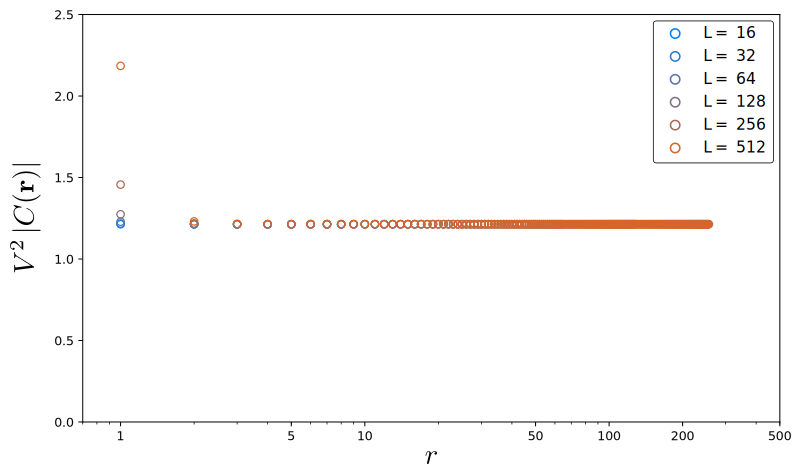
\includegraphics[width=0.8\linewidth]{./chapter07/HoneycombBondBondT=10.pdf}
	\caption{
		High-temperature bond-bond correlation function times squared system size calculated numerically for a number of system sizes on the honeycomb lattice in the ground state flux sector.
	}
	\label{fig:chapter07_6_3BondBondHighTemp}
\end{figure}
%

This analysis, of course, has ignored the thermal fluctuations of the gauge field for simplicity.
The author speculates that the $T \rightarrow \infty$ limit still holds for an arbitrary gauge configuration, however, in order to properly investigate the fate of bond-bond correlations at finite temperatures, one must include these fluctuations.


%
%
%%%%%%%%%%%%%%%%%%%%%%%%%%%%%%%%%%%%%%%%%%%%%%%%%%%%%%%%%%%%%%%%%%%%%%%%%%%%%%%%%%%%%%%%
\section{Summary and outlook}
\label{section:chapter07_Summary}
%%%%%%%%%%%%%%%%%%%%%%%%%%%%%%%%%%%%%%%%%%%%%%%%%%%%%%%%%%%%%%%%%%%%%%%%%%%%%%%%%%%%%%%%
%
%
The work reported in this chapter is the subject of ongoing study and, thus, leaves several questions open without unequivocal answers.
There are, however, a number of successes reported here as well.
This chapter began with a recapitulation of some well-known results about the Kitaev model for classical $O(3)$ spins.
In the classical model, the ground state manifold corresponds to an extensively degenerate number of dimer configurations where each spin is perfectly aligned with one of its nearest-neighbors.
The resulting classical spin liquid phase yields spin-spin correlations which vanish beyond nearest-neighbor spins due to the disordered nature of the dimer configurations.
By mapping to a hardcore dimer model and then to a coarse-grained field theory, the ground state manifold has been shown to be in a so-called Coulomb phase.
Thus it is argued on rather general grounds that bond-bond correlations in the classical Kitaev model should decay as a power law $C(\br) \sim 1/r^D$, where $D$ is the dimension of the lattice.

In the quantum model, spin-spin correlations similarly vanish beyond nearest-neighbors due to the conservation of \ZZ~fluxes.
Furthermore, the bond-bond correlation function also decays algebraically so long as the system is in a gapless spin liquid phase, otherwise it decays exponentially.
Rather than depending only on the dimension of the underlying lattice as is the case for the classical model, the decay exponent of the quantum model also depends intimately on the nature of the gapless excitations of the spin liquid.
A general trend is observed that the greater the dimension of the nodal manifold, the slower the decay of correlations.

Bond-bond correlations were calculated numerically for a number of both two- and three-dimensional lattices.
Additionally, the bond-bond correlation function was evaluated analytically in the long-wavelength limit for both the square-octagon and honeycomb lattices, showing good agreement with the numerics.
Although a detailed analysis has not yet been performed for the three-dimensional lattices, knowledge from the analysis of the two-dimensional lattices allowed for some general remarks to be made which are in qualitative agreement with the numerical data.